% Wersja źródłowa: audyt II, jednostka 18
\setcounter{section}{17}
\section{Funkcje testowe i ścisłe granice induktywne}
\label{sec:funkcje-testowe18}

\subsection{Funkcje o ustalonym zwartym nośniku}

W całym rozdziale zakładamy, że $d\ge1$, $\Omega\subseteq\R^d$
jest niepustym zbiorem otwartym, a $\K\in\{\R,\C\}$.
Dla $f\in C^\infty(\Omega;\K)$ definiujemy jego \emph{nośnik}
przez $\supp f=\overline{\{x\in\Omega:f(x)\ne0\}}^{\,\Omega}$,
tj. domknięcie względne w $\Omega$. Zapis $K\Subset\Omega$
oznacza, że $K$ jest zwartym podzbiorem $\Omega$.

\begin{definicja}[Przestrzeń $\mathcal D_K(\Omega)$]
\label{def:DK18}
Dla każdego zwartego $K\Subset\Omega$ kładziemy
\[
 \mathcal D_K(\Omega;\K)=\{\varphi\in C^\infty(\Omega;\K):
 \supp\varphi\subseteq K\}.
\]
Wyposażamy tę przestrzeń w topologię wyznaczoną przez seminormy
\[p_m(\varphi)=\max_{|\alpha|\le m}\sup_{x\in\Omega}
|\partial^\alpha\varphi(x)|,\qquad m\in\N_0.\]
Supremum jest skończone: wszystkie pochodne znikają poza $K$.
Jeżeli $\operatorname{int}K=\varnothing$, to $\mathcal D_K=\{0\}$.
\end{definicja}

\begin{twierdzenie}[Struktura etapów]
\label{thm:DK-frechet18}
Dla każdego zwartego $K\Subset\Omega$ przestrzeń
$\mathcal D_K(\Omega;\K)$ jest przestrzenią Fr\'echeta.
Jeżeli $K\subseteq L\Subset\Omega$ są zwarte, to
$\mathcal D_K$ jest domkniętą podprzestrzenią $\mathcal D_L$,
a włożenie $\mathcal D_K\hookrightarrow\mathcal D_L$
jest izomorfizmem na swój obraz z topologią względną.
\end{twierdzenie}
\begin{proof}
Z poprzedniego rozdziału wiemy, że
$C^\infty(\Omega;\K)$ jest przestrzenią Fr\'echeta.
Przestrzeń $\mathcal D_K$ jest w niej domknięta:
przy zbieżności $\varphi_j\to\varphi$ w $C^\infty(\Omega)$
i $\varphi_j\in\mathcal D_K$ mamy $\varphi(x)=0$ dla
$x\in\Omega\setminus K$, więc $\supp\varphi\subseteq K$.
Topologia względna na $\mathcal D_K$ pokrywa się z topologią
wyznaczoną przez $p_m$, ponieważ dla funkcji wspartych w $K$
wszystkie pochodne znikają poza $K$ i $p_m=p_{K,m}$
w oznaczeniach poprzedniego rozdziału.
Domknięta podprzestrzeń przestrzeni Fr\'echeta jest przestrzenią
Fr\'echeta. Ten sam argument, zastosowany do $K\subseteq L$,
daje domkniętość $\mathcal D_K$ w $\mathcal D_L$;
seminormy $p_m$ są na obu etapach określone tym samym wzorem.
\end{proof}

\begin{definicja}[Algebraiczna przestrzeń funkcji testowych]
\label{def:D-algebraic18}
Oznaczamy przez $\mathcal D(\Omega;\K)=C_c^\infty(\Omega;\K)$
przestrzeń wszystkich funkcji gładkich o zwartym nośniku.
Jeśli $(K_n)_{n\ge1}$ jest wyczerpaniem zwartymi zbiorami,
$K_n\subseteq\operatorname{int}K_{n+1}$ i każdy zwarty
$K\Subset\Omega$ jest zawarty w pewnym $K_n$, to
$\mathcal D(\Omega)=\bigcup_{n\ge1}\mathcal D_{K_n}(\Omega)$.
Takie wyczerpanie skonstruowano w
wcześniejszym lemacie o wyczerpaniu zwartym.
\end{definicja}

\subsection{Topologia granicy induktywnej}

\begin{definicja}[Lokalnie wypukła granica induktywna]
\label{def:LF18}
Niech $(E_n,\tau_n)$ będzie rosnącym ciągiem przestrzeni
lokalnie wypukłych nad $\K$, gdzie każde włożenie
$i_n:E_n\hookrightarrow E_{n+1}$ jest liniowe i ciągłe.
Na $E=\bigcup_nE_n$ rozważamy \emph{najsilniejszą lokalnie
wypukłą topologię}, dla której wszystkie odwzorowania
$E_n\hookrightarrow E$ są ciągłe. Oznaczamy ją
$\operatorname{ind}_n E_n$ i nazywamy topologią granicy induktywnej.
Jeżeli $E_n$ są przestrzeniami Fr\'echeta, otrzymujemy
przestrzeń typu $(LF)$; granica jest \emph{ścisła}, jeśli
każde $E_n$ ma topologię względną z $E_{n+1}$ i jest w nim
podprzestrzenią domkniętą.
\end{definicja}

\begin{twierdzenie}[Konstrukcja przez seminormy i własność uniwersalna]
\label{thm:LF-universal18}
Niech $E=\bigcup_nE_n$, gdzie każde $E_n$ jest przestrzenią
lokalnie wypukłą, a włożenia są ciągłe. Rozważmy rodzinę
$\mathcal P$ wszystkich seminorm $p:E\to[0,\infty)$ takich,
że $p|_{E_n}$ jest ciągła dla każdego $n$.
Topologia generowana przez $\mathcal P$ jest topologią
granicy induktywnej. Dla dowolnej przestrzeni lokalnie
wypukłej $F$ i odwzorowania liniowego $T:E\to F$ mamy
\[
 T\text{ jest ciągłe}\quad\Longleftrightarrow\quad
 T|_{E_n}:E_n\to F\text{ jest ciągłe dla każdego }n.
\]
\end{twierdzenie}
\begin{proof}
Dla $p\in\mathcal P$ włożenie $E_n\hookrightarrow E$ jest
ciągłe w topologii wyznaczonej przez $p$, więc również
w topologii wszystkich tych seminorm. Niech $\rho$ będzie
inną lokalnie wypukłą topologią na $E$, dla której włożenia
są ciągłe. Każda seminorma ciągła dla $\rho$ należy do
$\mathcal P$, gdyż jej ograniczenie do $E_n$ jest ciągłe.
Stąd $\rho$ jest nie silniejsza od naszej topologii.
Dla ostatniej równoważności wystarczy zastosować ten
argument do seminorm $q\circ T$, gdzie $q$ przebiega
wszystkie ciągłe seminormy na $F$.
\end{proof}

\begin{definicja}[Standardowa topologia $\mathcal D(\Omega)$]
\label{def:D-LF18}
Na $\mathcal D(\Omega;\K)$ przyjmujemy topologię
\[
 \mathcal D(\Omega;\K)
   =\operatorname{ind}_{n\to\infty}\mathcal D_{K_n}(\Omega;\K),
\]
gdzie $(K_n)$ jest wyczerpaniem z
Definicji~\ref{def:D-algebraic18}. Jest to \emph{standardowa
topologia funkcji testowych}. Nie należy jej utożsamiać
ani z topologią podprzestrzeni dziedziczoną po
$C^\infty(\Omega)$, ani automatycznie z końcową topologią
w kategorii wszystkich przestrzeni topologicznych.
\end{definicja}

\begin{stwierdzenie}[Niezależność od wyczerpania]
\label{prop:D-independence18}
Dwa wyczerpania $\Omega$ zbiorami zwartymi współkońcowe
wśród zwartych podzbiorów $\Omega$ prowadzą do tej samej
topologii na $\mathcal D(\Omega)$, nawet jeśli nie mają
identycznych wyrazów.
\end{stwierdzenie}
\begin{proof}
Niech $(K_n)$, $(L_j)$ będą takimi wyczerpaniami.
Seminorma $p$ na $\mathcal D(\Omega)$ jest ciągła na
każdym $\mathcal D_{K_n}$ wtedy i tylko wtedy, gdy jest
ciągła na każdym $\mathcal D_{L_j}$: dla ustalonego $K_n$
istnieje $L_j$ zawierający $K_n$, a ograniczenie seminormy
ciągłej na $\mathcal D_{L_j}$ do $\mathcal D_{K_n}$ jest
ciągłe. W drugą stronę argument jest symetryczny.
Korzystamy z Twierdzenia~\ref{thm:LF-universal18}.
\end{proof}

\begin{twierdzenie}[Topologia na każdym etapie i oddzielanie punktów]
\label{thm:D-stage18}
Dla dowolnego zwartego $K\Subset\Omega$ topologia względna
indukowana na $\mathcal D_K$ przez $\mathcal D(\Omega)$
jest topologią jego przestrzeni Fr\'echeta.
Ponadto $\mathcal D(\Omega)$ jest lokalnie wypukłą
przestrzenią liniowo-topologiczną Hausdorffa.
\end{twierdzenie}
\begin{proof}
Ciągłość włożenia $\mathcal D_K\to\mathcal D$ mówi, że
topologia względna nie jest silniejsza od topologii
$\mathcal D_K$. Dla każdego $m\in\N_0$ określmy na
całej $\mathcal D$ seminormę
$p_m(\varphi)=\max_{|\alpha|\le m}\sup_{x\in\Omega}
|\partial^\alpha\varphi(x)|$. Jej ograniczenie do
każdego $\mathcal D_{K_n}$ jest ciągłe, a zatem $p_m$
jest ciągła na $\mathcal D$ z
Twierdzenia~\ref{thm:LF-universal18}. Seminormy te
wyznaczają topologię względną $\mathcal D_K$, stąd
otrzymujemy także nierówność w przeciwnym kierunku.
Ponieważ $p_0(\varphi)>0$ dla $\varphi\ne0$, topologia
jest Hausdorffa; lokalna wypukłość wynika z konstrukcji.
\end{proof}

\begin{uwaga}[Przestrzeń dualna topologiczna]
\label{rem:D-dual18}
Własność uniwersalna jest szczególnie użyteczna dla
funkcjonałów: odwzorowanie liniowe $T:\mathcal D(\Omega)\to\K$
jest ciągłe wtedy i tylko wtedy, gdy każde ograniczenie
$T|_{\mathcal D_K}$ jest ciągłe. Ponieważ $\mathcal D_K$
ma topologię seminorm $p_m$, równoważnie: dla każdego
$K\Subset\Omega$ istnieją $C_K>0$ i $m_K\in\N_0$ takie, że
\[
 |T(\varphi)|\le C_K p_{m_K}(\varphi)
 \qquad(\varphi\in\mathcal D_K(\Omega)).
\]
Wielkości $C_K$ i $m_K$ mogą zależeć od $K$.
To będzie podstawowe kryterium w teorii dystrybucji.
\end{uwaga}


\begin{przyklad}[Dystrybucja o nieograniczonym rzędzie globalnym]
\label{ex:variable-order18}
Niech $\Omega=\R$. Dla $\varphi\in\mathcal D(\R)$ określamy
$T(\varphi)=\sum_{n=1}^\infty \varphi^{(n)}(n)$.
Suma jest skończona dla każdej $\varphi$, gdyż tylko skończenie
wiele liczb naturalnych może należeć do zwartego nośnika.
Na każdym $\mathcal D_K$ funkcjonał jest sumą skończonej
liczby ciągłych ewaluacji pochodnych, więc $T$ jest ciągły
na $\mathcal D(\R)$.

Nie istnieje jednak jeden rząd $m$ właściwy dla wszystkich
kompaktów, nawet z osobno dobranymi stałymi $C_K$.
Ustalmy $m$ i wybierzmy liczbę całkowitą $n>m$.
Niech $\chi\in C_c^\infty((-1/4,1/4))$ będzie równa $1$
w pobliżu zera, a $\psi(t)=t^n\chi(t)$. Dla $0<\varepsilon<1$
kładziemy $\varphi_\varepsilon(x)=\varepsilon^n
\psi((x-n)/\varepsilon)$. Wszystkie te funkcje mają
nośniki w jednym zwartym przedziale wokół $n$, przy czym
$T(\varphi_\varepsilon)=\psi^{(n)}(0)=n!$,
natomiast $p_m(\varphi_\varepsilon)\to0$.
To wyklucza oszacowanie z jednym globalnie ustalonym $m$.
\end{przyklad}

\subsection{Zbiory ograniczone, ciągi i pełna zupełność}

\begin{twierdzenie}[Dokładne kryterium ograniczoności]
\label{thm:D-bounded18}
Niech $B\subseteq\mathcal D(\Omega;\K)$. Następujące
warunki są równoważne:
\begin{enumerate}
\item $B$ jest ograniczony w topologii $\mathcal D(\Omega)$;
\item istnieje zwarty $K\Subset\Omega$, który zawiera
nośniki wszystkich $\varphi\in B$, a ponadto dla każdego
$m\in\N_0$ zachodzi $\sup_{\varphi\in B}p_m(\varphi)<\infty$.
\end{enumerate}
\end{twierdzenie}
\begin{proof}
Jeżeli $B\subseteq\mathcal D_K$ jest ograniczony w
$\mathcal D_K$, to jego obraz przez ciągłe włożenie
jest ograniczony w $\mathcal D$.

Na odwrót, niech $B$ będzie ograniczony w $\mathcal D$.
Ponieważ każda seminorma $p_m$ z dowodu
Twierdzenia~\ref{thm:D-stage18} jest ciągła, mamy
$\sup_{\varphi\in B}p_m(\varphi)<\infty$.
Pozostaje wykazać wspólność nośnika. Załóżmy przeciwnie,
że $B$ nie zawiera się w żadnym $\mathcal D_{K_n}$.
Dla każdego $n$ wybierzmy $\varphi_n\in B$ oraz
$x_n\in\Omega\setminus K_n$ z $\varphi_n(x_n)\ne0$.
Punkty $x_n$ opuszczają każdy zwarty podzbiór $\Omega$,
ponieważ wyczerpanie jest współkońcowe. Możemy więc
wybrać gładkie funkcje nieujemne $\theta_n$, równe $1$
w $x_n$, o nośnikach tworzących rodzinę lokalnie skończoną
w $\Omega$. Ustalmy $a_n>n/|\varphi_n(x_n)|$ i określmy
$w(x)=1+\sum_{n\ge1}a_n\theta_n(x)$. Suma jest lokalnie
skończona, zatem $w$ jest dodatnią funkcją gładką.
Seminorma $p_w(\varphi)=\sup_{x\in\Omega}w(x)|\varphi(x)|$
jest skończona dla każdej funkcji testowej. Dla ustalonego
$K$ mamy $p_w|_{\mathcal D_K}\le(\sup_Kw)p_0$, więc
z Twierdzenia~\ref{thm:LF-universal18} wynika jej ciągłość
na $\mathcal D$. Jednak $p_w(\varphi_n)>n$,
co przeczy ograniczoności $B$. Wobec tego istnieje
$K_n$ zawierający wszystkie nośniki, a oszacowania
$p_m$ kończą dowód.
\end{proof}

\begin{twierdzenie}[Zbieżność ciągów funkcji testowych]
\label{thm:D-sequences18}
Dla ciągu $(\varphi_j)\subseteq\mathcal D(\Omega;\K)$
i $\varphi\in\mathcal D(\Omega;\K)$ następujące warunki
są równoważne:
\begin{enumerate}
\item $\varphi_j\to\varphi$ w topologii $\mathcal D(\Omega)$;
\item istnieje zwarty $K\Subset\Omega$ zawierający
$\supp\varphi$ i wszystkie $\supp\varphi_j$ oraz
$p_m(\varphi_j-\varphi)\to0$ dla każdego $m\in\N_0$.
\end{enumerate}
\end{twierdzenie}
\begin{proof}
Ciąg zbieżny wraz z granicą jest zbiorem ograniczonym
w dowolnej przestrzeni liniowo-topologicznej: dla ustalonego
otoczenia zera najpierw wchłaniamy jego wyrazy od pewnego
indeksu, a następnie skończenie wiele pozostałych.
Twierdzenie~\ref{thm:D-bounded18} daje wspólny zwarty $K$.
Ponieważ topologia na $\mathcal D_K$ jest względna,
zbieżność w $\mathcal D$ oznacza zbieżność w $\mathcal D_K$,
a tę charakteryzują seminormy $p_m$.
Implikacja odwrotna wynika z ciągłości
$\mathcal D_K\hookrightarrow\mathcal D$.
\end{proof}

\begin{wniosek}[Zupełność sekwencyjna]
\label{cor:D-seqcomplete18}
Każdy ciąg Cauchy'ego w $\mathcal D(\Omega;\K)$ jest
zbieżny w tej przestrzeni.
\end{wniosek}
\begin{proof}
Każdy ciąg Cauchy'ego jest ograniczony w przestrzeni lokalnie
wypukłej: dla każdej ciągłej seminormy jego wartości tworzą
ciąg Cauchy'ego, a więc ograniczony.
Wybieramy wspólny $K$ z
Twierdzenia~\ref{thm:D-bounded18}. Ograniczenia topologii
na $\mathcal D_K$ i $\mathcal D$ są jednakowe, więc ciąg
jest Cauchy'ego w przestrzeni Fr\'echeta $\mathcal D_K$;
tam ma granicę, do której zbiega również w $\mathcal D$.
\end{proof}

\begin{twierdzenie}[Zupełność $\mathcal D(\Omega)$]
\label{thm:D-complete18}
Przestrzeń $\mathcal D(\Omega;\K)$ jest zupełna:
każdy filtr Cauchy'ego względem jej kanonicznej struktury
jednostajnej jest zbieżny. W szczególności jest zupełną
ścisłą przestrzenią typu $(LF)$.
\end{twierdzenie}
\begin{proof}
Przeprowadzimy dowód dla ogólnej rosnącej sumy
$E=\bigcup_nE_n$ przestrzeni zupełnych lokalnie wypukłych,
która ma topologię granicy induktywnej i indukuje na
każdym $E_n$ topologię wyjściową. W naszym przypadku
$E_n=\mathcal D_{K_n}$, a wszystkie te własności już
udowodniono.

Niech $\mathcal F$ będzie filtrem Cauchy'ego w $E$.
Przez $\mathcal N$ oznaczmy filtr otoczeń zera, a przez
$\mathcal G$ filtr generowany przez zbiory $F+V$,
$F\in\mathcal F$, $V\in\mathcal N$. Filtr $\mathcal G$
jest filtrem Cauchy'ego, słabszym od $\mathcal F$.
Pokażemy, że dla pewnego $n$ każdy element $\mathcal G$
przecina $E_n$.

Załóżmy przeciwnie. Dla każdego $n$ istnieją
$F_n\in\mathcal F$ i absolutnie wypukłe otoczenie
$V_n$ zera w $E$ takie, że
$(F_n+V_n)\cap E_n=\varnothing$. Zastępując $V_n$
odpowiednimi skończonymi przekrojami, możemy zakładać
$V_{n+1}\subseteq V_n$. Definiujemy
$W=\operatorname{aco}(\bigcup_n(V_n\cap E_n))$,
gdzie $\operatorname{aco}$ oznacza absolutnie wypukłą
otoczkę zbioru. Zbiór $W$ jest absolutnie wypukły,
pochłaniający w $E$, a dla każdego $n$ zbiór
$W\cap E_n$ zawiera otoczenie $V_n\cap E_n$ zera w $E_n$.
Z konstrukcji topologii granicy induktywnej wynika, że
$W$ jest otoczeniem zera: jego funkcjonał Minkowskiego
jest ciągły na każdym etapie i zatem na $E$.

Dla ustalonego $n$ składniki sumy z indeksami $k\le n$
należą do $E_n$, natomiast te z $k>n$ należą do $V_n$.
Dlatego $W\subseteq E_n+V_n$ i
$(F_n+W)\cap E_n=\varnothing$.
Ponieważ $\mathcal F$ jest filtrem Cauchy'ego, istnieje
$F_0\in\mathcal F$ takie, że $F_0-F_0\subseteq W$.
Wybierzmy $x\in F_0$; należy on do pewnego $E_n$.
Istnieje $y\in F_0\cap F_n$, bo oba zbiory należą do
filtru $\mathcal F$. Ale
$x=y+(x-y)\in(F_n+W)\cap E_n$, sprzeczność.

Zatem istnieje $n$ takie, że każdy element $\mathcal G$
przecina $E_n$. Przecięcia tych elementów z $E_n$
wyznaczają filtr Cauchy'ego na $E_n$, ponieważ topologia
$E_n$ jest indukowana przez $E$, a $\mathcal G$
jest Cauchy'ego. Zupełność $E_n$ daje jego granicę
$x\in E_n$. Punkt $x$ jest punktem skupienia filtru
$\mathcal G$ w $E$. Filtr Cauchy'ego mający punkt skupienia
jest zbieżny do tego punktu: dla dowolnego otoczenia
$U$ zera bierzemy $V$ z $V+V\subseteq U$ oraz
$G\in\mathcal G$ z $G-G\subseteq V$; skoro
$(x+V)\cap G\ne\varnothing$, to $G\subseteq x+U$.
Stąd $\mathcal G\to x$, a ponieważ $\mathcal F$ jest
silniejszy, również $\mathcal F\to x$.
\end{proof}

\subsection{Dlaczego topologia \texorpdfstring{$\mathcal D$}{D} jest istotna?}

\begin{przyklad}[Ucieczka nośników]
\label{ex:escaping18}
Wybierzmy ciąg niezerowych funkcji $\psi_n\in\mathcal D(\Omega)$
mających nośniki poza $K_n$. Każda taka funkcja istnieje,
ponieważ $\Omega\setminus K_n$ jest niepustym zbiorem otwartym.
Dla dowolnego zwartego $K\Subset\Omega$ i ustalonego $m$
mamy $p_{K,m}(\psi_n)=0$ dla dostatecznie dużych $n$.
Zatem $\psi_n\to0$ w $C^\infty(\Omega)$.
Nie zachodzi jednak $\psi_n\to0$ w $\mathcal D(\Omega)$,
ponieważ nośniki nie mieszczą się w żadnym wspólnym
zbiorze zwartym. Właśnie dlatego topologia funkcji testowych
jest ściśle silniejsza od topologii względnej z $C^\infty$.
\end{przyklad}

\begin{twierdzenie}[Niemetryzowalność]
\label{thm:D-nonmetric18}
Dla każdego niepustego otwartego $\Omega\subseteq\R^d$,
$d\ge1$, przestrzeń $\mathcal D(\Omega;\K)$ z jej
standardową topologią nie jest metryzowalna.
\end{twierdzenie}
\begin{proof}
Każda podprzestrzeń $E_n=\mathcal D_{K_n}$ jest domknięta
w $\mathcal D$: istotnie,
$E_n=\bigcap_{x\in\Omega\setminus K_n}\{\varphi:\varphi(x)=0\}$,
a ewaluacje $\varphi\mapsto\varphi(x)$ są ciągłe
na każdym etapie, więc i na $\mathcal D$.
Każde $E_n$ jest właściwe i jako podprzestrzeń liniowa
ma puste wnętrze w $\mathcal D$.
Gdyby $\mathcal D$ miała przeliczalną malejącą bazę
otoczeń zera $(U_n)$, moglibyśmy wybrać
$\varphi_n\in U_n\setminus E_n$. Wtedy
$\varphi_n\to0$, lecz nośniki $\varphi_n$ nie mieściłyby
się w żadnym wspólnym zbiorze zwartym, wbrew
Twierdzeniu~\ref{thm:D-sequences18}.
\end{proof}

\begin{twierdzenie}[Względna zwartość zbiorów ograniczonych]
\label{thm:D-Montel18}
Każdy zbiór ograniczony $B\subseteq\mathcal D(\Omega;\K)$
jest względnie zwarty w standardowej topologii.
\end{twierdzenie}
\begin{proof}
Z Twierdzenia~\ref{thm:D-bounded18} istnieje zwarty $K$
taki, że $B\subseteq\mathcal D_K$ i wszystkie seminormy
$p_m$ są jednostajnie ograniczone na $B$.
Przedłużmy funkcje z $\mathcal D_K$ zerem poza $\Omega$
do funkcji gładkich na $\R^d$. Dla każdej pochodnej
$\partial^\alpha$ pochodne rzędu $|\alpha|+1$ mają
jednostajną normę supremum, toteż rodzina
$\{\partial^\alpha\varphi:\varphi\in B\}$ jest
jednostajnie ograniczona i równociągła na $\R^d$
(z twierdzenia o wartości średniej). Na zwartym $K$
możemy zastosować twierdzenie Arzel\`a--Ascoliego.
Wybierając kolejno podciągi dla przeliczalnej rodziny
wielowskaźników i stosując argument diagonalny,
uzyskujemy podciąg dowolnego ciągu elementów $B$,
którego wszystkie pochodne są jednostajnie zbieżne na $K$.
Poza $K$ są zerowe. Z zupełności $\mathcal D_K$
wynika istnienie granicy w $\mathcal D_K$, a więc także
w $\mathcal D$. Skoro $\mathcal D_K$ jest metryzowalna,
sekwencyjna względna zwartość daje względną zwartość
w $\mathcal D_K$, a ciągłe włożenie do $\mathcal D$
przenosi zwartość domknięcia.
\end{proof}

\begin{stwierdzenie}[Naturalne operatory na funkcjach testowych]
\label{prop:D-operators18}
Niech $a\in C^\infty(\Omega;\K)$ i
$\alpha\in\N_0^d$. Odwzorowania
$\varphi\mapsto\partial^\alpha\varphi$ oraz
$\varphi\mapsto a\varphi$ są ciągłymi operatorami
liniowymi $\mathcal D(\Omega)\to\mathcal D(\Omega)$.
Dla $f\in L^1_{\mathrm{loc}}(\Omega;\K)$ odwzorowanie
$T_f(\varphi)=\int_\Omega f(x)\varphi(x)\,\mathrm d\lambda_d(x)$
jest ciągłym funkcjonałem liniowym na $\mathcal D(\Omega)$.
\end{stwierdzenie}
\begin{proof}
Każdy z dwóch pierwszych operatorów zachowuje
$\mathcal D_K$ i na nim jest ciągły: z reguły Leibniza
na $K$ dostajemy oszacowania za pomocą skończenie
wielu seminorm $p_m$. Ciągłość na $\mathcal D$ wynika
z Twierdzenia~\ref{thm:LF-universal18}.
Dla $\varphi\in\mathcal D_K$ mamy
$|T_f(\varphi)|\le
\bigl(\int_K|f(x)|\,\mathrm d\lambda_d(x)\bigr)p_0(\varphi)$,
a więc każde ograniczenie $T_f|_{\mathcal D_K}$
jest ciągłe. Ponownie stosujemy własność uniwersalną.
\end{proof}

\begin{center}
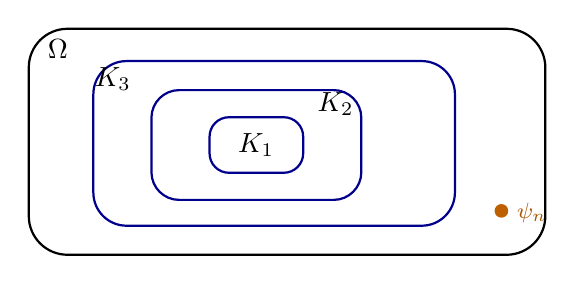
\begin{tikzpicture}[scale=0.82]
 \draw[thick,rounded corners=14pt] (-4,-1.7) rectangle (4,1.8);
 \draw[thick,rounded corners=12pt,blue!55!black] (-3.0,-1.25) rectangle (2.6,1.3);
 \draw[thick,rounded corners=10pt,blue!55!black] (-2.1,-0.85) rectangle (1.15,0.85);
 \draw[thick,rounded corners=7pt,blue!55!black] (-1.2,-0.43) rectangle (0.25,0.43);
 \node at (-0.48,0) {$K_1$};
 \node at (0.75,0.64) {$K_2$};
 \node at (-2.70,1.02) {$K_3$};
 \node at (-3.55,1.49) {$\Omega$};
 \fill[orange!75!black] (3.32,-1.02) circle (3pt);
 \node[orange!65!black,anchor=west,font=\footnotesize] at (3.41,-1.05) {$\psi_n$};
\end{tikzpicture}

\small\emph{Schemat:} funkcje testowe mogą mieć nośniki poza
kolejnymi zbiorami zwartymi, a wtedy nie tworzą ciągu zbieżnego
w topologii $\mathcal D(\Omega)$, nawet jeśli zbiegają do zera
w $C^\infty(\Omega)$.
\end{center}

\begin{uwaga}[Przejście do dystrybucji]
\label{rem:D-distributions-next18}
W kolejnym rozdziale zdefiniujemy przestrzeń dystrybucji
$\mathcal D'(\Omega)$ jako przestrzeń dualną topologiczną
$\mathcal D(\Omega)$. Podstawowe oszacowania funkcjonałów
uzyskaliśmy już w Uwadze~\ref{rem:D-dual18}; będziemy też
odróżniać topologię słabą-* od topologii zbieżności
jednostajnej na zbiorach ograniczonych funkcji testowych.
\end{uwaga}
